\documentclass[acmsmall,screen,nonacm]{acmart}

\let\Bbbk\relax
\usepackage{amsmath,amssymb}
\usepackage{amsthm}
\newtheorem{remark}{Remark}
\usepackage{booktabs}
\usepackage{listings}
\usepackage{tikz}
\usetikzlibrary{arrows.meta,positioning,fit,calc}

%% Lean listing style
\definecolor{leankeyword}{RGB}{0,0,255}
\definecolor{leancomment}{RGB}{0,128,0}
\definecolor{leanstring}{RGB}{163,21,21}
\lstdefinelanguage{Lean}{
  morekeywords={theorem,lemma,def,inductive,structure,where,import,open,namespace,end,section,variable,by,have,exact,rcases,intro,apply,sorry,noncomputable,instance,class,abbrev,Type,Prop,Exists,Nonempty},
  sensitive=true,
  morecomment=[l]{--},
  morecomment=[n]{/-}{-/},
  morestring=[b]",
}
\lstset{
  language=Lean,
  basicstyle=\ttfamily\small,
  keywordstyle=\color{leankeyword}\bfseries,
  commentstyle=\color{leancomment}\itshape,
  stringstyle=\color{leanstring},
  breaklines=true,
  columns=flexible,
  showstringspaces=false,
  tabsize=2,
  frame=single,
  numbers=none,
  xleftmargin=1em,
  xrightmargin=1em,
}

\newcommand{\lean}[1]{\lstinline!#1!}
\newcommand{\N}{\mathbb{N}}

\title{Beyond Boolean Intersections: A Verified Bisimulation and Trace Decompiler\\for Causal Graphs}

\author{Lucia Yizi Zhang}
\affiliation{%
  \institution{Shanghai Lixin University of Accounting and Finance}
  \country{China}
}



\setlength{\headheight}{19pt}
\begin{document}

\begin{abstract}
We mechanize a verified bisimulation between two standard characterizations of
d-separation in Lean~4, expose a concrete counterexample to unrestricted
equivalence, and build a constructive decompiler that synthesizes
exploitability-certificate witnesses from graph reachability alone.

The two characterizations---trail blocking~\cite{pearl2009causality} and
moralized ancestral-graph separation~\cite{lauritzen1996graphical}---have been
treated as unconditionally equivalent in the literature.  We machine-check a
counterexample showing that the equivalence fails when an endpoint node lies in
the conditioning set~$Z$, identify the minimal repair
($\text{DisjointSets}\,X\,Y\,Z$, an affine ownership constraint), and discharge
both directions of the corrected equivalence with no proof debt.

The forward direction is a \emph{certified trace optimizer}: it compiles any
active trail through a Bayes-ball state machine into a compressed moral-graph
walk, certifying soundness under the exact domain restriction that repairs
equivalence.  The reverse direction is a \emph{constructive decompiler of
semantic flow}: from moral-graph reachability we reconstruct an explicit
active-trail witness, including a proved bad-collider normalization
(\lean{route_improves_of_bad}) that strictly decreases a well-founded
measure.  Both directions compose into a closed equivalence on the
pairwise-disjoint domain (\lean{dSeparated_iff_dSeparates}); the graph core
carries no proof debt.

The verified bisimulation serves as a zero-sorry graph-semantic foundation for
certified Shannon-style leakage bounds.  The local
\lean{InfoTheoryBridge.lean} file contains two intentional scaffold stubs
restating results from a separate anonymized artifact~\cite{companionqif};
two named technical debts in the quantitative chain (the Verma--Pearl
factorization derivation and the dual KL capacity sufficiency theorem) are
identified in Section~\ref{sec:related} but do not affect the graph core.
\end{abstract}
\maketitle

\section{Introduction}\label{sec:intro}

Formalizing both standard characterizations of d-separation in
Lean~4's dependent type system yields a mechanized counterexample: the
unrestricted equivalence between Pearl's trail-blocking predicate and
Lauritzen's moralized ancestral-graph separation is \emph{false}.  When an
endpoint node lies in the conditioning set~$Z$, the moral-graph construction
deletes that endpoint while the trail predicate still admits the one-edge trail
that has no internal triple.

The counterexample lives on the simplest possible directed acyclic graph: a chain of three nodes
$0 \to 1 \to 2$. We show in Section~\ref{sec:counterexample} that setting $X = \{0\}$, $Y = \{1\}$, and $Z = \{0\}$ breaks equivalence: moral-graph separation unconditionally deletes $Z$ (disconnecting $X$ from $Y$), while trail blocking leaves the one-edge trail $0 \to 1$ unblocked.

We mechanize this discrepancy and its repair, treating the two
characterizations not as interchangeable definitions but as a \emph{verified
bisimulation} between two semantic layers:
\begin{itemize}
  \item an \textbf{operational semantics} of active trails (the ``execution''
    layer of information flow);
  \item a \textbf{static analysis} of moralized-graph reachability (the
    ``compiled'' layer).
\end{itemize}
The forward direction (soundness) is a \emph{certified trace optimizer}
that compiles an operational trace into static reachability evidence.  The
reverse direction (completeness) is a \emph{constructive decompiler of semantic
flow}: it reconstructs a concrete execution witness---an exploitability
certificate for the information leak---from static reachability alone.  The
counterexample says exactly that the two languages are \emph{not} bisimilar
without a well-typed domain restriction.

\subsection{Contributions}

Contributions:
\begin{enumerate}
  \item We machine-check a concrete counterexample
    (\lean{dsep_complete_endpoint_in_Z_counterexample}) showing that
    unrestricted equivalence between trail blocking and moral-graph separation
    is false, identify the minimal repair ($\text{DisjointSets}\,X\,Y\,Z$ as
    an affine ownership constraint), and prove that no counterexample survives
    the repair.
  \item We formalize both d-separation characterizations in Lean~4 as a
    three-layer stack: type-safe graph syntax, certified intermediate
    representations (\lean{MAGWalk}, \lean{StaticRoute}, \lean{OpenTrace},
    \lean{ActiveRoute}), and witness-extraction pipelines.
  \item We mechanize the \textbf{certified trace optimizer} (soundness): an
    explicit compilation pipeline
    $\text{Trail} \to \text{BayesBallPath} \to \text{MAGWalk} \to \allowbreak \text{Reachable}$,
    certified by node-survival proofs.
  \item We mechanize the \textbf{constructive decompiler of semantic flow}
    (witness-producing completeness): a decompilation pipeline
    $\text{Reachable} \to \text{StaticRoute} \to \text{OpenTrace} \to \allowbreak \text{ActiveRoute} \to \exists\,\text{Trail},\;\neg\text{isBlocked}$.
    Every stage is type-indexed and constructive, including a proved
    bad-collider normalization (\lean{exists_split}, \lean{ancestor_escape},
    \lean{route_improves_of_bad}) that strictly decreases a well-founded
    measure.  The reverse pipeline carries no \lean{sorry}.
  \item We close the \textbf{full equivalence}
    (\lean{dSeparated_iff_dSeparates}): on the pairwise-disjoint domain,
    moral-graph separation holds if and only if every trail is blocked, with
    both directions discharged by the optimizer and the decompiler.
  \item We bridge the graph core to a certified Shannon leakage bound via a
    companion anonymized artifact~\cite{companionqif}. The explicit scaffold
    \lean{InfoTheoryBridge.lean} restates the companion-proved capacity bounds. 
    The remaining technical debts bounding this claim are localized to the
    quantitative pipeline and do not affect the graph-semantic core 
    (discussed in Section~\ref{sec:related}).
\end{enumerate}

The graph results are available as a standalone Lean~4 package.  The
decompiler produces not a mere existence proof but a computational
witness---a $\Sigma$-type containing the actual trail and the proof that it is
unblocked.

\section{A Three-Layer Architecture}\label{sec:architecture}

Our formal development uses three layers mirroring a verified compiler's architecture.

\subsection{Layer 1: Type-Safe Graph Syntax}

Nodes are natural numbers, edges are a finite set of ordered pairs
($\mathrm{Finset}\,(\N \times \N)$), and acyclicity is well-foundedness of the
edge relation.  The key safety invariant is
\lean{DisjointSets X Y Z}, which requires pairwise disjointness of the three
node sets.  In the language of substructural types, this is an \emph{affine
ownership constraint}: the conditioned variables $Z$ are borrowed by the query
and cannot alias the source $X$ or sink $Y$.
As planned future work for the POPL track---not part of this artifact---we
target a first-order surface calculus with an explicit environment and no
higher-order binders, so the metatheory would stay focused on queries rather
than substitution-heavy closure machinery.  In that planned layer, surface
graphs would carry a rank certificate for acyclicity, checked locally and then
elaborated into intrinsic \lean{DAG}s via \lean{DAG.ofRank}.

\begin{lstlisting}[caption={DAG structure and safety predicate}]
structure DAG where
  nodes : Finset \N
  edges : Finset (\N \times \N)
  edges_subset : \forall {u v}, (u,v) \in edges -> u \in nodes \wedge v \in nodes
  acyclic : WellFounded fun u v => (u,v) \in edges

def DisjointSets (X Y Z : Finset \N) : Prop :=
  Disjoint X Y \wedge Disjoint X Z \wedge Disjoint Y Z
\end{lstlisting}

\subsection{Layer 2: Certified Intermediate Representations}

Between operational trails and graph reachability sits a family of IRs that
preserve just enough structure for certified translation.

\paragraph{MAGWalk.} A compressed walk language equivalent to moral-graph
reachability.  It has three constructors: reflexivity, a single directed or
reversed edge (\lean{MAGWalk.single}), and a ``moral jump'' over an active
collider (\lean{MAGWalk.jump}).  The collider node is skipped, which is why
compression is correct.

\paragraph{StaticRoute.} A type-valued decompiler IR that keeps the witness
hidden by graph reachability.  Each step is either a forward edge, a backward
edge, or a moral jump storing the common child:

\begin{lstlisting}[caption={Static route IR (excerpt)}]
inductive StaticStep (G : DAG) (X Y Z : Finset \N) : \N -> \N -> Type where
  | directForward  (hEdge : G.HasEdge u v) ...
  | directBackward (hEdge : G.HasEdge v u) ...
  | moralJump (huw : G.HasEdge u w) (hvw : G.HasEdge v w)
      (hw : w \in G.ancestralSubgraphNodes (X \cup Y \cup Z)) ...
\end{lstlisting}

\paragraph{OpenTrace.} The compiler target before converting to an active route.
Each \lean{cons} node stores its oriented DAG traversal \emph{and} a local
non-blocking proof, making \lean{OpenTrace} a type-valued certificate that every
junction is $Z$-open.

\subsection{Layer 3: Witness-Extraction Pipelines}

The two pipelines are summarized in Figure~\ref{fig:pipeline}.

\begin{figure}[ht]
\centering
\resizebox{\textwidth}{!}{
\begin{tikzpicture}[
  node distance=1.8cm and 2.4cm,
  every node/.style={align=center, font=\small},
  box/.style={draw, rounded corners, minimum width=2.2cm, minimum height=0.9cm, fill=blue!5},
  arrow/.style={-{Stealth}, thick},
  label/.style={font=\scriptsize\itshape, above, sloped}
]
  % Forward (optimizer)
  \node[box] (trail) {Active trail\\$t : \text{Trail}\,G\,x\,y$};
  \node[box, right=of trail] (bb) {Bayes-ball path\\$p : \text{BayesBallPath}$};
  \node[box, right=of bb] (mag) {MAGWalk\\$w : \text{MAGWalk}\,G\,X\,Y\,Z$};
  \node[box, right=of mag] (reach) {Graph reachability\\$\text{Reachable}_{G'}\,x\,y$};

  \draw[arrow] (trail) -- node[label]{lift} (bb);
  \draw[arrow] (bb) -- node[label]{compress} (mag);
  \draw[arrow] (mag) -- node[label]{embed} (reach);

  % Reverse (decompiler)
  \node[box, below=1.2cm of reach] (rreach) {$\text{Reachable}_{G'}\,x\,y$};
  \node[box, left=of rreach] (rstatic) {StaticRoute\\$r : \text{StaticRoute}$};
  \node[box, left=of rstatic] (ropen) {OpenTrace\\$o : \text{OpenTrace}$};
  \node[box, left=of ropen] (ractive) {ActiveRoute\\$a : \text{ActiveRoute}$};
  \node[box, left=of ractive] (rtrail) {$\exists\,\text{Trail},\;\neg\text{isBlocked}$};

  \draw[arrow, dashed] (rreach) -- node[label]{decompile} (rstatic);
  \draw[arrow, dashed] (rstatic) to [out=110, in=70, looseness=5] node[label]{normalize} (rstatic);
  \draw[arrow, dashed] (rstatic) -- node[label]{compile} (ropen);
  \draw[arrow, dashed] (ropen) -- node[label]{bridge} (ractive);
  \draw[arrow, dashed] (ractive) -- node[label]{realize} (rtrail);

  % Bracket labels
  \node[above=0.3cm of trail, font=\bfseries\small] {Forward: Certified Trace Optimizer};
  \node[below=0.3cm of rtrail, font=\bfseries\small] {Reverse: Decompilation of Semantic Flow};
\end{tikzpicture}
}
\caption{The two witness-extraction pipelines.  Solid arrows: forward
(soundness).  Dashed arrows: reverse (completeness).  Every arrow, including
the \emph{normalize} step, is a total constructive function in Lean; the
normalize step is a proved bad-collider minimization
(Section~\ref{sec:reverse}).}
\Description{The two witness-extraction pipelines showing forward and reverse logic.}
\label{fig:pipeline}
\end{figure}

\section{Background: The Two Criteria}\label{sec:background}

\subsection{Trail Blocking (Operational Semantics)}

An undirected \emph{trail} from $x$ to $y$ in a DAG $G$ is a finite walk that may
follow edges forward or backward.  A consecutive triple $a \to b \to c$ or
$a \leftarrow b \to c$ is a \emph{non-collider}; $a \to b \leftarrow c$ is a
\emph{collider}.  A triple is \emph{blocked} by $Z$ if:
\begin{itemize}
  \item it is a non-collider whose middle node is in $Z$; or
  \item it is a collider whose middle node and all descendants are disjoint from $Z$.
\end{itemize}
A trail is \emph{blocked} by $Z$ if some internal triple is blocked.  Then $Z$
\emph{d-separates} $X$ from $Y$ in the trail sense if every trail from $X$ to $Y$
is blocked by $Z$.

\subsection{Moral Graph Separation (Static Analysis)}

The \emph{ancestral subgraph} of $S$ is the subgraph induced by all ancestors of
nodes in $S$.  Its \emph{moral graph} is obtained by (1)~forgetting edge
directions and (2)~connecting all co-parents (pairs of nodes with a common child).
The \emph{d-separation graph} is the moral graph of the ancestral subgraph of
$X \cup Y \cup Z$ with $Z$ removed.  Then $Z$ d-separates $X$ from $Y$ in the
graph sense if no node of $X$ is connected to any node of $Y$ in this graph.

\subsection{Textbook Equivalence and Its Caveat}

Standard references state that the two criteria are equivalent under the implicit
assumption that $X$, $Y$, and $Z$ are pairwise disjoint.  In applications,
however, the disjointness precondition is often omitted.  Our counterexample
(Section~\ref{sec:counterexample}) shows that this omission is not benign.

\section{The Bug in the Math Textbook}\label{sec:counterexample}

Our counterexample lives on the simplest non-trivial DAG:

\begin{center}
\begin{tikzpicture}[node distance=1.5cm, every node/.style={circle,draw,minimum size=0.7cm}]
  \node (n0) {$0$};
  \node (n1) [right of=n0] {$1$};
  \node (n2) [right of=n1] {$2$};
  \draw[-{Stealth}] (n0) -- (n1);
  \draw[-{Stealth}] (n1) -- (n2);
\end{tikzpicture}
\end{center}

Let $X = \{0\}$, $Y = \{1\}$, $Z = \{0\}$.

\begin{theorem}[Endpoint-in-$Z$ counterexample]\label{thm:counterexample}
There exists a DAG $G$ and finite sets $X, Y, Z \subseteq \N$ such that
$G$ d-separates $X$ from $Y$ in the moral-graph sense, but $Z$ does \emph{not}
d-separate $X$ from $Y$ in the trail-blocking sense.
\end{theorem}

\begin{lstlisting}[caption={Mechanized counterexample}]
theorem dsep_complete_endpoint_in_Z_counterexample :
    \exists (G : DAG) (X Y Z : Finset \N),
      DAG.dSeparated G X Y Z \wedge \neg dSeparates G X Y Z := by
  refine <chain3, {0}, {1}, {0}, ?_, ?_>
  ...
\end{lstlisting}

\paragraph{Why the disagreement happens.} Trail blocking only inspects
\emph{internal} triples.  The one-edge trail $0 \to 1$ has no internal triple at
all, so nothing can block it.  By contrast, the moral-graph construction deletes
$Z$ unconditionally; since $0 \in Z$, the edge $(0,1)$ disappears from the
moralized graph, and $0$ and $1$ are disconnected.

\paragraph{The standard repair.} If we require $X \cap Z = \emptyset$ and
$Y \cap Z = \emptyset$, the start node of any trail is never deleted, and the
endpoint caveat disappears.

\section{The Certified Trace Optimizer}\label{sec:forward}

Under $\text{DisjointSets}\,X\,Y\,Z$, we mechanize the soundness direction:
\[
\text{DAG.dSeparated}(G,X,Y,Z) \;\Longrightarrow\; \text{dSeparates}(G,X,Y,Z).
\]

The proof follows a three-stage compilation pipeline.

\paragraph{Stage 1: Trail $\to$ Bayes-ball path.} If a trail $t$ from $x \in X$
to $y \in Y$ is not blocked by $Z$, and $x \notin Z$ (guaranteed by
$\text{Disjoint}\,X\,Z$), then we lift $t$ to an explicit Bayes-ball state path.
The construction is by induction on the trail, analyzing each directional triple
to show that the Bayes-ball state machine can traverse it.

\begin{lstlisting}[caption={Trail to Bayes-ball path}]
def bayesBallPath_of_active_trail_outOf
    (t : Trail G u v) (h_active : \neg t.isBlocked Z)
    (huZ : u \notin Z) :
    \Sigma final_dir, BayesBallPath G Z (u, outOf) (v, final_dir)
\end{lstlisting}

\paragraph{Stage 2: Certified membership.} The Bayes-ball path contains
intermediate states that must ``survive'' deletion of $Z$.  We prove a certified
version that guarantees every \lean{RequiredState} node belongs to the
d-separation graph nodes:

\begin{lstlisting}[caption={Certified Bayes-ball path}]
def bayesBallPathCert_of_active_trail_outOf
    (t : Trail G u v) (h_active : \neg t.isBlocked Z)
    (huZ : u \notin Z)
    (huA : u \in G.ancestralSubgraphNodes (X \cup Y \cup Z))
    (hvD : v \in G.dSeparationGraphNodes X Y Z) :
    \Sigma final_dir, {p : BayesBallPath ... //
      \forall {q}, BayesBallPath.RequiredState p q ->
        q.1 \in G.dSeparationGraphNodes X Y Z}
\end{lstlisting}

\paragraph{Stage 3: Compress to MAGWalk.} A Bayes-ball path is a sequence of
single-edge steps.  The \lean{compress} algorithm scans it with a two-step
window: ordinary non-collider windows become a \lean{MAGWalk.single}, while
active-collider windows $(a,\_) \to (b,\text{into}) \to (c,\text{outOf})$ become
a single \lean{MAGWalk.jump} over the collider $b$.  The collider itself need not
survive deletion of $Z$, which is why this compression is correct.

\begin{theorem}[Soundness]\label{thm:soundness}
For any DAG $G$ and pairwise-disjoint finite sets $X, Y, Z \subseteq \N$,
if $G$ d-separates $X$ from $Y$ in the moral-graph sense, then every trail
from $X$ to $Y$ is blocked by $Z$.
\end{theorem}

\begin{lstlisting}[caption={Top-level soundness theorem}]
theorem dSeparated_of_dSeparated_disjoint
    (hXYZ : DisjointSets X Y Z)
    (hsep : DAG.dSeparated G X Y Z) : dSeparates G X Y Z
\end{lstlisting}

\section{Decompilation of Semantic Flow}\label{sec:reverse}

The reverse direction is the decompiler: from $\neg\text{DAG.dSeparated}$ it
constructively reconstructs an active-trail witness---an exploitability
certificate showing that the conditioning set $Z$ fails to block the flow.
The pipeline is:
\[
\begin{aligned}
\text{Reachable}
&\;\to\; \text{StaticRoute}
\;\to\; \text{NormalizedStaticRoute} \\
&\;\to\; \text{OpenTrace}
\;\to\; \text{ActiveRoute}
\;\to\; \exists\,\text{Trail},\;\neg\text{isBlocked}.
\end{aligned}
\]

\subsection{From Reachability to StaticRoute}

Graph reachability is a \lean{Prop}-valued relation that hides the structure of
each step.  We introduce \lean{StaticStep} and \lean{StaticRoute} as type-valued
evidence: a \lean{StaticRoute} is an explicit list of directed edges, reversed
edges, and moral jumps, each carrying the witness needed for later stages.

\begin{lstlisting}[caption={Reachability to static route}]
theorem nonemptyStaticRoute_of_dSeparationGraph_reachable
    (h : (G.dSeparationGraph X Y Z).Reachable u v) :
    Nonempty (StaticRoute G X Y Z u v)
\end{lstlisting}

\subsection{Normalization: Eliminating Bad Colliders}

A ``bad collider'' is a collider window whose middle node and all descendants are
disjoint from $Z$.  Such a collider is blocked, so it must be eliminated.  Normalization may change endpoints: if a bad collider leaks
ancestry into $X$ or $Y$, we reroute the prefix or suffix to a different node in
that set.

We package static routes as endpoint-carrying witnesses
(\lean{StaticRouteWitness}) and define a bad-collider count \lean{routeBadCount}.
The minimization is a \lean{Nat.find} wrapper: if every nonzero-count witness can
be strictly improved, a zero-count witness exists.

\begin{lstlisting}[caption={Bad-collider minimization wrapper}]
theorem normalized_route_exists_of_improves
    (hwit : \exists w : StaticRouteWitness G X Y Z, True)
    (himprove : \forall w, routeBadCount w \neq 0 ->
      \exists w', routeBadCount w' < routeBadCount w) :
    \exists w, routeBadCount w = 0
\end{lstlisting}

The improvement obligation is discharged by the core normalization theorem,
which is fully proved (no \lean{sorry}):

\begin{lstlisting}[caption={Strict improvement for non-normalized routes}]
theorem route_improves_of_bad
    (w : StaticRouteWitness G X Y Z) (hbad : routeBadCount w \neq 0) :
    \exists w' : StaticRouteWitness G X Y Z,
      routeBadCount w' < routeBadCount w
\end{lstlisting}

The proof is a short dispatcher over three established lemmas.
\lean{exists_split} extracts the first bad collider as a \lean{Split} carrying a
zero-bad prefix and a count bound.  \lean{ancestor_escape} shows the bad child's
leaked ancestry must reach a node in $X$ or $Y$ (its descendant cone misses
$Z$, so it cannot dead-end).  \lean{bad_child_survives} and
\lean{escape_path_survives} prove that the rerouted escape chain stays inside
the d-separation graph nodes.  Reattaching the escape chain---backward into $X$
or forward into $Y$---removes a moral jump of cost $1$ and adds chains of cost
$0$; the strict decrease then follows by
\texttt{countBadColliders\_backwardEscape\_}\allowbreak\texttt{append\_suffix\_lt} (resp.\
\texttt{countBadColliders\_prefix\_append\_}\allowbreak\texttt{forwardEscape\_lt}) and \lean{omega}.  As a
deliberate design choice, the witness endpoints may change: rerouting is allowed
to land on a \emph{different} node of $X$ or $Y$, which is what makes the escape
construction total.

\subsection{From Zero-Bad StaticRoute to OpenTrace to ActiveRoute}

A static route with zero bad colliders compiles directly to an \lean{OpenTrace},
because every junction is locally open:

\begin{lstlisting}[caption={Zero-bad compiler}]
theorem openTrace_of_countBadColliders_zero
    (hzero : countBadColliders arrival route = 0) :
    Nonempty (\Sigma finalDir, OpenTrace G Z (x, arrival) (y, finalDir))
\end{lstlisting}

The \lean{OpenTrace} is then converted to a \lean{BayesBallPath} and wrapped as
an \lean{ActiveRoute}.  Finally, \lean{ActiveRoute.to_activeTrail} yields the
existential witness:

\begin{lstlisting}[caption={Final decompiler theorem}]
theorem activeWitness_of_not_dSeparated
    (hnot : \neg DAG.dSeparated G X Y Z) : ActiveWitness G X Y Z
\end{lstlisting}

The result is a constructive $\Sigma$-type containing the actual nodes $x \in X$,
$y \in Y$, the final direction, and the active route.

\subsection{The Closed Equivalence}

Composing the optimizer (Section~\ref{sec:forward}) and the decompiler yields
the full equivalence on the well-typed domain---the bisimulation
statement: on pairwise-disjoint $X,Y,Z$, the operational and static languages
agree exactly.

\begin{lstlisting}[caption={Full d-separation equivalence (no proof debt)}]
theorem dSeparated_iff_dSeparates
    (hXYZ : DisjointSets X Y Z) :
    DAG.dSeparated G X Y Z <-> dSeparates G X Y Z
\end{lstlisting}

\begin{remark}[Verification status]\label{rem:status}
The full Lean development typechecks (\lean{lake build}).  The graph-semantic
core---both directions of \lean{dSeparated_iff_dSeparates} and the entire
reverse synthesis stack---contains no \lean{sorry}.  The only \lean{sorry}s in
the package are two \emph{intentional} scaffold stubs in
\lean{InfoTheoryBridge.lean} (Section~\ref{sec:related}), which are out of
scope for the equivalence claims.
\end{remark}

\section{The PL Dictionary: Reframing Causal Graphs}\label{sec:dictionary}

To situate this work for a POPL audience, we reframe traditional causal-graph
vocabulary in programming-languages terms:

\begin{table}[ht]
\centering
\small
\begin{tabular}{ll}
\toprule
\textbf{Causal Inference} & \textbf{PL Framing} \\
\midrule
DAG & Dataflow AST / Dependency Graph Syntax \\
$\text{DisjointSets}\,X\,Y\,Z$ & Affine ownership constraint (no aliasing of $Z$) \\
Active Trail & Operational trace of semantics \\
MAGWalk & Reachability abstract IR (compressed moral-graph walk) \\
Collider Jump (\lean{MAGWalk.jump}) & Peephole optimization / semantic fold \\
Trail $\to$ BayesBallPath & Typestate tracking \\
BayesBallPath $\to$ MAGWalk & Certified trace optimizer \\
StaticRoute $\to$ OpenTrace $\to$ ActiveRoute & Semantic-flow decompiler / exploitability-certificate generator \\
Cut-Set / Mutual Information & Quantitative Information Flow (QIF) capacity bounds \\
\bottomrule
\end{tabular}
\caption{Reframing causal-graph concepts for a POPL audience.}
\label{tab:dictionary}
\end{table}

\section{Related Work}
\label{sec:related}

Our mechanization sits at the intersection of causal inference, mechanized probabilistic semantics, and verified compilation. We briefly survey the most closely related lines of work.

\paragraph{Mechanized Causal Inference and D-Separation.}
Formalizing the graph-theoretic foundations of causal inference is an active area of research. Recently, Chancelier, De Lara, and Heymann~(2024) \cite{chancelier2024conditional} mechanized d-separation as a binary relation using Coq and MathComp/SSReflect, providing a relational-algebraic treatment of graphical separation. Parallel to our work, Anna Zhang~(2025) \cite{coqci2025} formalized the semantics of conditional independence and d-separation in Coq, bridging structural properties with function-based definitions for experimental design.

Both developments adopt standard mathematical formulations without exposing the implicit textbook domain caveats. Our work contributes the first formalized counterexample and repair (the endpoint caveat) for the gap between syntactic trails and moralized node-deletion. We also shift from purely relational verification to a constructive bisimulation that generates executable IRs (e.g., \lean{OpenTrace}), optimized in Lean~4 for computational witness synthesis.

\paragraph{Categorical and Topological D-Separation.}
Fritz and Klingler~(2023) \cite{fritz2023dseparation}, extending work by Fritz and Liang~(2023) \cite{fritz2023free}, abstracted d-separation using string diagrams in Markov categories. Their framework bypasses moralization, reading conditional independence directly from topological connectedness in a generalized measure-theoretic space. Our approach is complementary: Markov categories provide a general topological theory, while our artifact targets the legacy operational graph definitions (moral graphs and trace trails) implemented in existing software. By defining \lean{DisjointSets} as an affine ownership type, we show that classical d-separation behaves like a resource-restricted syntax within a broader categorical structure.

\paragraph{Verified Trace Bisimulation and Witness Extraction.}
The forward pipeline (soundness) translates unbounded trace semantics into a compressed step-relation (\lean{MAGWalk}), analogous to the semantics-preserving translations in Leroy's CompCert~(2009) \cite{leroy2009formal}. The reverse pipeline (completeness) deterministically unwinds reachability into a certified active trail, resembling Necula's Proof-Carrying Code~(1997) \cite{necula1997proof}: instead of returning a boolean assertion of an information leak, our decompiler synthesizes an explicit, machine-checkable exploitability certificate. This provides a graph-theoretic substrate for future verified static analyzers of quantitative information flow.

\subsection{Quantitative Information-Flow Bridge \& Technical Debts}

\paragraph{Certified Shannon bounds.} Security analysis has moved from
non-interference (``0 or 1'') to measuring leakage in bits.  The verified
bisimulation here supplies the graph-semantic front end for such bounds: a
closed d-separation equivalence licenses replacing a conditional-independence
premise by a checked graph property in a cut-set capacity argument.  The full
finite chain is
\[
\text{d-separation} \;\Rightarrow\; \text{conditional independence}
\;\Rightarrow\; \text{conditional DPI} \;\Rightarrow\; \text{cut-set bound}.
\]

This arXiv artifact does not import the quantitative project.  Instead,
\lean{InfoTheoryBridge.lean} states the first bridge as an explicit local
scaffold: the conditional-independence predicate \lean{ConditionalIndependence}
and the bridge theorem
\lean{dSeparation_implies_conditional_independence}
are stubbed alongside placeholder structures \lean{FinitePMF} and
\lean{MarkovCompatible}.  This scaffold carries exactly two intentional
\lean{sorry}s, and it restates results proved in the separate anonymized
artifact \cite{companionqif}.

Engineering note: the graph artifact and the quantitative artifact are two
physically separate Lake projects with near-isomorphic DAG definitions and no
shared imports yet. The two \lean{sorry}s in this repository's
\lean{InfoTheoryBridge.lean} file are a port placeholder for the proved
semantic bridge in the cited anonymous artifact.

\paragraph{Remaining Technical Debts.} This section separates proved theorem
chains from remaining work in the broader pipeline:
\begin{enumerate}
  \item \textbf{Debt~1: Structural Verma--Pearl derivation.}  The companion
    artifact proves the semantic bridge \lean{factorizes_dsep_implies_cond_indep} 
    under a stated \lean{FactorizesOverDAG} hypothesis. What remains open is the 
    structural derivation of \lean{FactorizesOverDAG} from a standard DAG 
    factorization theorem; it is a narrow algebraic gap, not a gap in the semantic 
    bridge theorem. (Sandbox implementation in \texttt{scratch\_markov.lean}; 
    pending integration.)
  \item \textbf{Debt~2: General capacity metatheorem (dual KL witness).}  The
    companion artifact proves concrete capacity certificates, including
    \lean{capacity_le_of_kkt}, and uses them in cut-set bounds.  A general
    Blahut--Arimoto/KKT concavity sufficiency theorem with a dual KL witness
    remains future work. (Sandbox implementation in \texttt{scratch\_dual.lean}; 
    pending integration.) The Gaussian-KL steps are carried as explicit external
    premises (\lean{AssumesFanoBound}, \lean{AssumesMissedCellBound}).
  \item \textbf{Surface calculus and certified decision procedure.}  The
    current artifact verifies the intrinsic \lean{DAG} core.  The planned
    first-order surface syntax, rank checker, elaboration soundness theorem,
    query conservativity theorem, and certified d-separation decision
    procedure are not yet mechanized.
\end{enumerate}

\section{Conclusion}\label{sec:conclusion}

A machine-checked counterexample shows that the two standard textbook
characterizations of d-separation disagree when an endpoint lies in the
conditioning set.  The minimal repair---$\text{DisjointSets}\,X\,Y\,Z$ as an
affine ownership constraint---recovers full equivalence.  We discharge both
directions: a certified trace optimizer (soundness) and a constructive,
witness-producing decompiler with proved bad-collider normalization
(completeness), composing into the closed theorem
\lean{dSeparated_iff_dSeparates} with no proof debt in the graph-semantic core.

The verified bisimulation grounds a certified Shannon leakage-bound pipeline
via a companion artifact. Two named technical debts in the quantitative 
pipeline are detailed in Section~\ref{sec:related}.



\bibliographystyle{ACM-Reference-Format}
\bibliography{references}

\end{document}
